\documentclass[../../../interview-questions.tex]{subfiles}

\begin{document}

\subsection{为什么Redis快}

Redis 的速度非常的快,单机的 Redis 就可以支撑每秒 10 几万的并发,相对于 MySQL 来说,性能是 MySQL(并发几百到几千)的几十倍。速度快的原因主要有几点:

\begin{enumerate}
    \item {\bf{基于内存}} 完全基于内存操作
    \item {\bf{高效的数据结构}} C 语言实现,优化过的数据结构,基于几种基础的数据结构,Redis 做了大量的优化,性能极高
    \item {\bf{合理的数据编码}}
    
\begin{figure}[htbp]
    \centering
    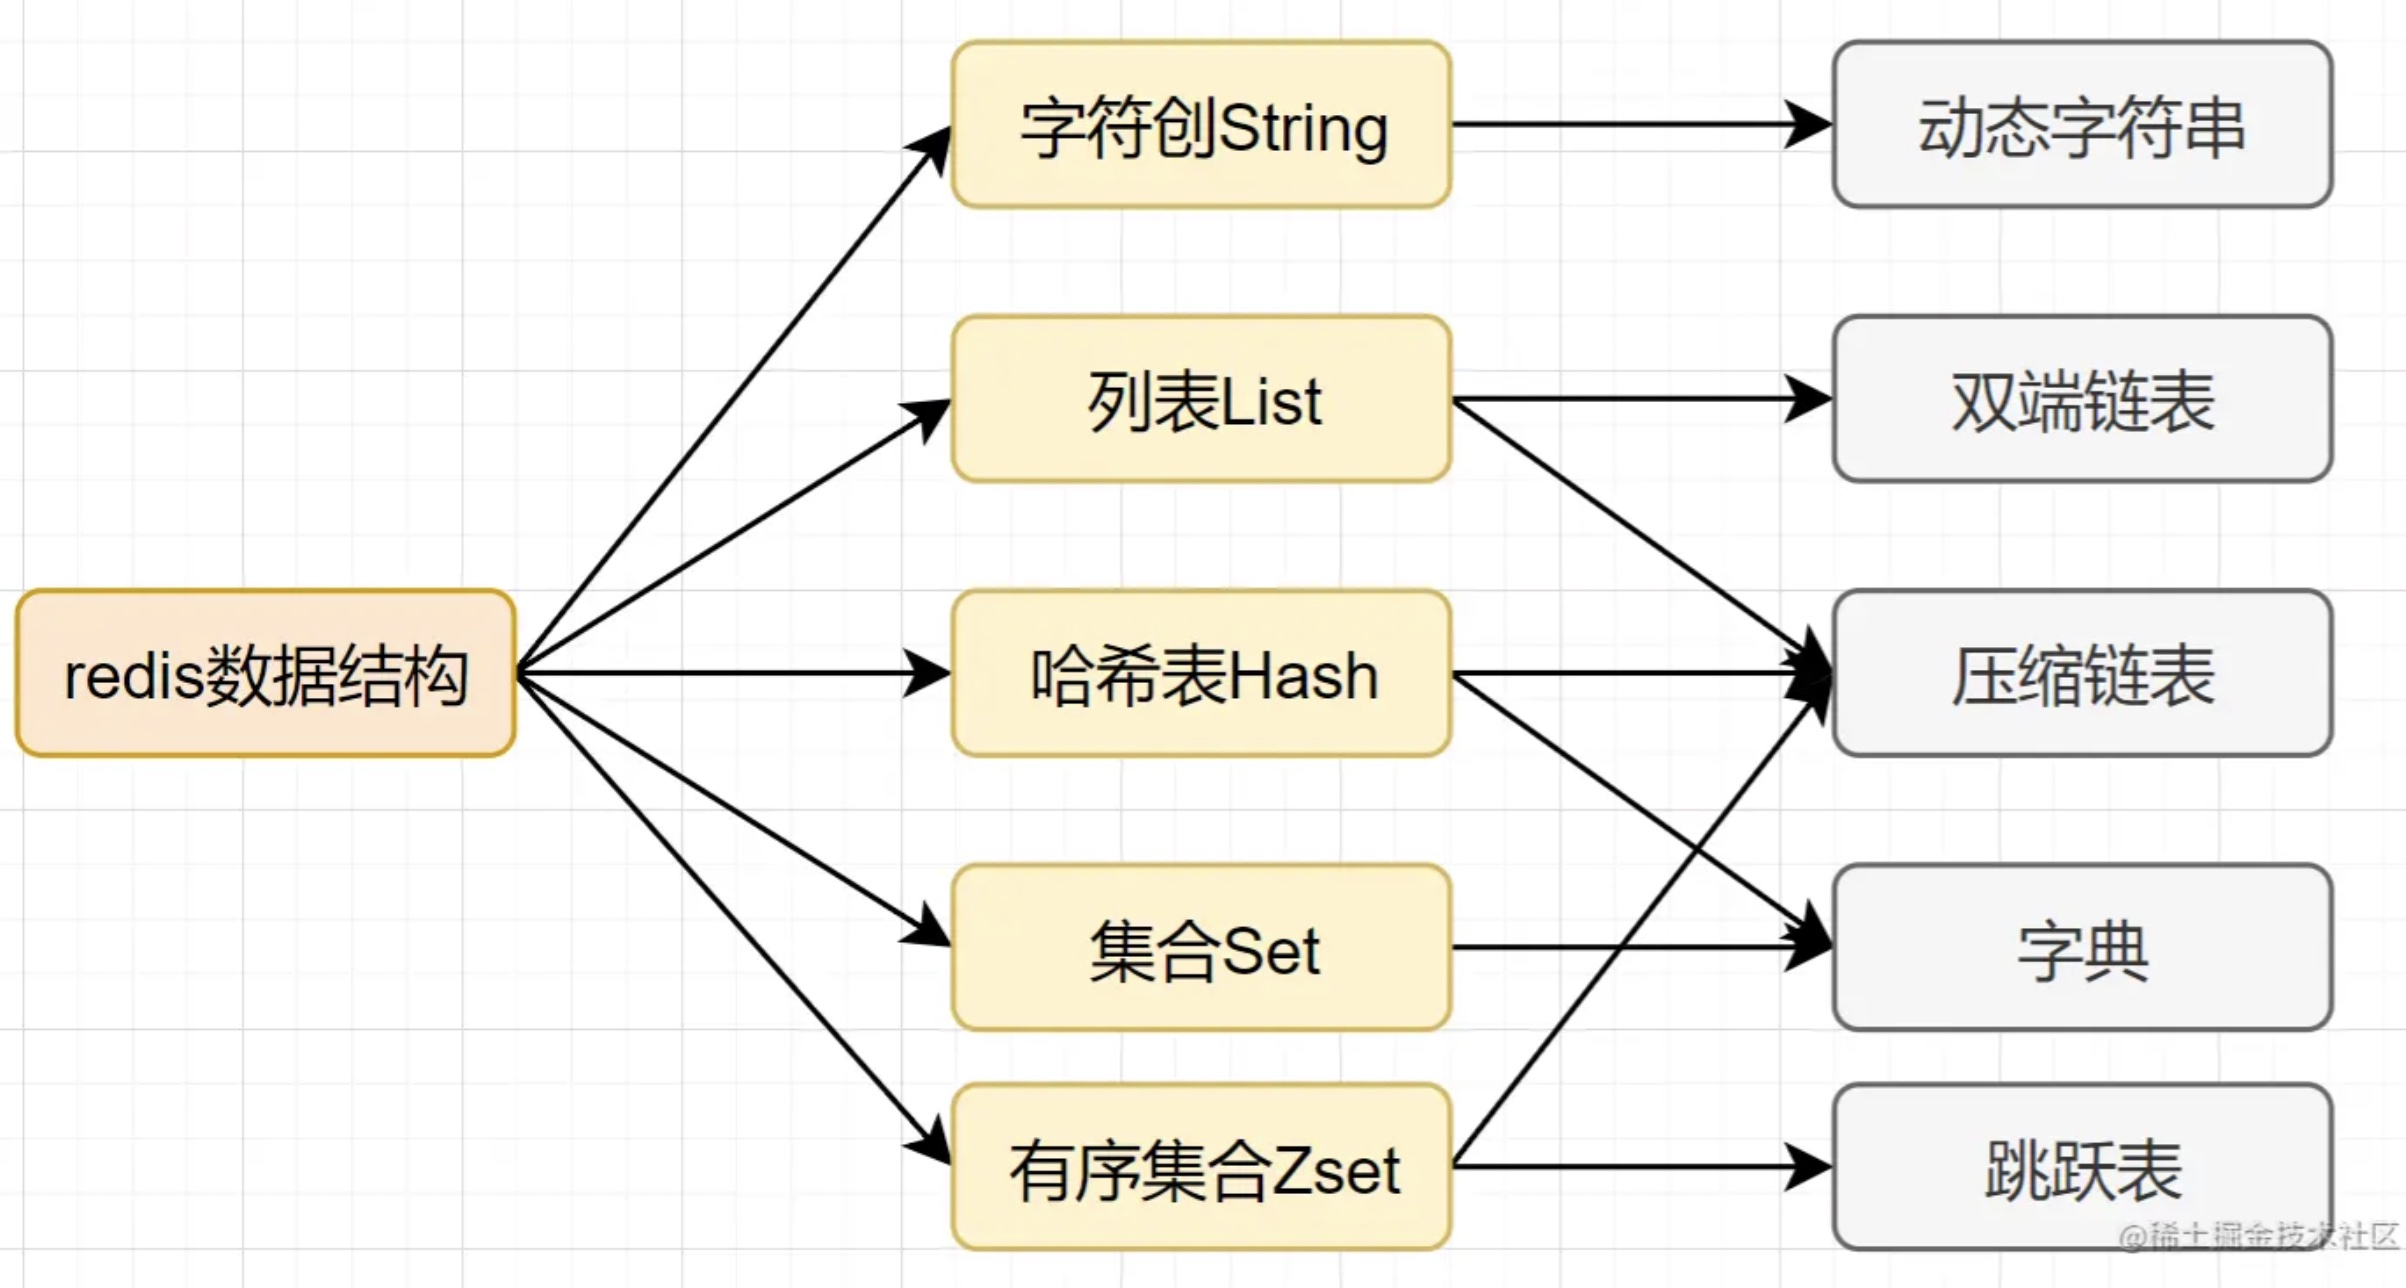
\includegraphics[scale=0.15]{redisdatastructure.jpg}
    \caption{Redis数据结构}
    \label{fig:redisdatastructure}
\end{figure}
    

    \item {\bf{合理的线程模型}} 使用单线程,无上下文的切换成本,基于非阻塞的 IO 多路复用机制。
    \item {\bf{虚拟内存机制}} 虚拟内存机制就是暂时把不经常访问的数据(冷数据)从内存交换到磁盘中,从而腾出宝贵的内存空间用于其它需要访问的数据(热数据)。通过VM功能可以实现冷热数据分离,使热数据仍在内存中、冷数据保存到磁盘。这样就可以避免因为内存不足而造成访问速度下降的问题。
\end{enumerate}

https://juejin.cn/post/6978280894704386079

\end{document}